\chapter{Theoretical Background}\label{sec:basics}

This chapter presents the theoretical background of this thesis. We will explain the foundations of quantitative information flow control and the different measures that are used to quantify information leakage. Furthermore, we will outline important aspects of (approximate) model counting, as well basic principles used in static (Q)IFC analyses \emph{Nildumu} and \emph{JOANA}, as both are used in our hybrid QIFC tool.

\section{Quantitative Information Flow Control}

Information flow control aims to guarantee the confidentiality of the secret input data of a program, by examining the flow of information through the program to public output channels, where the information would become accessible to an attacker.

There are different ways in which such information leakage might happen: Explicit information flows happen, when a secret values itself is written to a public channel or the information is copied to a variable that is later in leaked to a public channel. An example of a program is shown in figure \ref{fig:exEx}. Information leaks through implicit flows happen, when secret values affect the program's output through influencing the execution path. Figure \ref{fig:ifEx} shows a program snippet that contains an implicit flow. Additional to explicit and implicit flows, an attacker could gain information trough covert channels by observing a program's usage of different resources, such as time or memory \cite{smith07}.

Qualitative information flow analysis tries to prove the absence of explicit and implicit information flows, a property called \emph{non-interference}. For real world applications, leaking a certain amount of information is often required to build useful programs. In this case, the non-interference property is too strict. Instead, we wish to limit the amount of information that is leaked. Quantitative information flow analysis provides tools to measure how much information can be learned by an attacker about a program's secret inputs \cite{smith09}.

We consider the following scenario: Given a program \p, that accepts some input \In and produces some output \Out, how much information can an adversary \A learn about $H$, by observing \p and \Out?

\paragraph{Input program} We assume \p to be a sequential, deterministic program, that receives a set of inputs $\mathtt{H = \{h_1, ..., h_n\}}$ and produces a set of outputs $\mathtt{L = \{l_1, ..., l_m\}}$. We will write the sets of all possible inputs and outputs as $\mathcal{H}$ $\mathcal{L}$ respectively. Inputs are chosen based on a publicly known a priori probability distribution. The program text of \p is publicly known. A more detailed description of the input language we used, we refer to \ref{sec:inputLang}.

\paragraph{Security Lattice} Each element of \In and \Out is associated with an element of a security lattice, describing its confidentiality level. We use a lattice with two elements $\hat{l}$, for public values and $\hat{h}$ for secret values. If not otherwise specified, we consider all inputs to be high and all outputs to be low.
% Schneider -- nur high und low

\paragraph{Attacker Model} We consider an adversary \A that is able to observe the program text of \p and the resulting outputs on public channels. He or she is also aware of the set of program inputs and its underlying probability distribution. We assume the attacker is not able to extract any information through covert channels. The goal of the attacker is to guess the secret input of the program, using the information they can extract through observing the program's output.

%% standard def von min etropy aus smith paper funzt nicht für public inputs
%% new notion (min-entropy ???)
%% handbuch for quantitative information flow

% many leakage measures use average over all possible executions (min entropy, Shannon entropy)
% leakage can differ greatly between different executions --> example algorithm 1
% want to measure amount of information attacker has about the input after a single program execution

\begin{figure}
    \centering
    \begin{minipage}{.7\linewidth}
        \begin{algorithm}[H]
            \hspace*{\algorithmicindent} \textbf{Input} h: int \\
            \hspace*{\algorithmicindent} \textbf{Output} l: int
            \hspace*{1em}
            \begin{algorithmic}[1]
                \State $l: int \leftarrow h \: \% \: 10$
                \State leak(l)
            \end{algorithmic} 
        \end{algorithm}
\end{minipage}
\caption{Example for information leakage through explicit flows}
\label{fig:exEx}
\end{figure}

\begin{figure}
    \centering
    \begin{minipage}{.7\linewidth}
        \begin{algorithm}[H]
            \hspace*{\algorithmicindent} \textbf{Input} h: int \\
            \hspace*{\algorithmicindent} \textbf{Output} l: int
            \hspace*{1em}
            \begin{algorithmic}[1]
                \State $l: int \leftarrow 0$
                \If{$h == 42$}
                \State $l \leftarrow 1$
                \EndIf
                \State leak(l)
            \end{algorithmic} 
        \end{algorithm}
\end{minipage}
\caption{Example for information leakage through implicit flows}
\label{fig:ifEx}
\end{figure}

\subsection{Quantifying Information Flow}

In \cite{smith09}, Smith characterizes information leakage with the following equation:
\begin{center}
    Initial uncertainty = information leaked + remaining uncertainty.
\end{center}
In our scenario, the unknown value \In is the initial uncertainty, measured by some entropy measure. The remaining uncertainty is the entropy of \In after observing \Out. 

Because the programs we consider are deterministic, each program $p$ induces a mapping $\llbracket p \rrbracket: \mathcal{H} \longrightarrow \mathcal{L}$. From this mapping we can define an equivalence relation called the \emph{indistinguishability relation} as shown in definition \ref{def:ir}. The equivalence class of this relation are pre-images of the possible program outputs (see definition \ref{def:is}). When the adversary observes the value \Out, he knows that the secret input must be an element of $\mathcal{H}_mOut$. Thus, the bigger the size of $\mathcal{H}_mOut$, the less likely the adversary is, to guess the secret input in a single try \cite{backes09, smith09, alvim19}. 

\begin{definition}[Indistinguishability Relation]\label{def:ir}
        For each program $p$, we define the \emph{indistinguishability relation} $\thicksim$ over $\mathcal{H}$ as:
        \begin{center}
            $\forall \mIn, \mIn' \in \mathcal{H}: \mIn \thicksim  \mIn' \iff \llbracket p \rrbracket(\mIn) = \llbracket p \rrbracket(\mIn')$
        \end{center}
\end{definition}

\begin{definition}[Indistinguishability Set]\label{def:is}
    The indistinguishability set of a public output $\mOut \in \mathcal{L}$ of a program $p$ is given as:
    \begin{center}
        $\mathcal{H}_{\mOut} := \llbracket p \rrbracket^{-1} (\mOut) = \{ H \in \mathcal{H} \: | \: \llbracket p \rrbracket (\mIn) = \mOut \}$
    \end{center}
\end{definition}

\paragraph*{Measuring Leakage with Vulnerability}
A widely used measure for information leakage is \emph{vulnerability} and \emph{min-entropy} (\td{citations}). Following the definitions from \cite{smith09}, the vulnerability of a value $X$ describes `the worst case probability, that an adversary could guess the value of $X$ in one try.'

\begin{definition}[Vulnerability]\label{def:vul}
    Let $X$ be a random variables and $\mathcal{X}$ the set of possible values for $X$. The \emph{vulnerability} $V(X)$ is defined as
    \begin{center}
        $V(X) := \max\limits_{x \in \mathcal{X}} P[X = x]$
    \end{center}
\end{definition}

\begin{definition}[Min-Entropy]
    Using the same definitions as in \ref{def:vul}, the min-entropy of $X$ is given bx
    \begin{center}
        $H_\infty (X) := \log_2 \frac{1}{V(X)}$
    \end{center}
\end{definition}

\begin{definition}[Channel Capacity]
    
    Given a program $p$, the channel capacity of $p$ is the number of distinct outputs $|\mathcal{L}|$ than can be produced by $p$
\end{definition}

\td{finish}

\section{Program Representation}

\paragraph{Static Single Assignment}
Static single assignment (SSA) is a representation of the program, where every variable is assigned exactly once. If in the original program, a variable is written to more than once, a copy of the variable is created, that replaces the original one from that point in the program \cite{rosen88}.

\paragraph{Control Flow Graphs}
A control flow graph (CFG) is a graph, that represents all possible program execution traces via paths in the graph \cite{allen70}. They are widely used in compiler optimizations and static program analyses. The nodes of a CFG are a function's basic blocks, plus two special blocks \texttt{start} and \texttt{end}, that mark the single entry- and exit point of the function. An edge is inserted for every possible jump from one block to another. An example graph for the program from figure \ref{fig:ifEx} can be seen in \ref{fig:cfg}.

We use $\mbb_p$ for the set of all basic blocks of a program \p and $b_1, b_2, ...$ for the blocks themselves. With exception of the \texttt{start}- and \texttt{end}-block, every block in the CFG has at minimum one predecessor and one successor. In \ref{def:succPred} we define functions to access the predecessors and successors of a basic block, that we will use throughout this thesis. We assume all CFGs to have no critical edges (see \cite{dragoonBook}). This property can be assured by splitting critical edges with empty basic blocks, should they occur. 

\begin{definition}[CFG predecessors and successors]\label{def:succPred}
    The functions will return the set of predecessor and successor blocks respectively for the given basic block.
    \begin{center}
        $pred: \bb_p \longrightarrow 2^{\bb_p}$\\
        $succ: \bb_p \longrightarrow 2^{\bb_p}$
    \end{center}
    We assume for $pred(b)$ that the returned set of predecessors for $b$ is ordered and that the order corresponds to the arguments of any $\phi$-functions that might be present in $b$.
\end{definition}

\subsection{Program Dependence Graphs}
A program dependence graph (PDG) is an intermediate representation of a program that makes explicit the programs data and control dependencies. Its nodes are the programs statements and expressions and the edges represent the dependencies that exist between those \cite{ferrante87}. The Program Dependence Graph of \ref{fig:ifEx} is shown in figure \ref{fig:pdg}.

A data dependency edge between nodes $x$ and $y$ exists, if $x$ assigns a value that is used in the statement $y$.

A control dependency edge between nodes $x$ and $y$ exists, if the outcome of $x$ has influence on whether node $y$ will be executed.

Thus, a path $x \stackrel{*}{\rightsquigarrow } y$ between two nodes exists, if information can flow in the program from location $x$ to location $y$. Consequently, if there is no path, no information can flow between the two statements. This property makes PDGs a popular tool for information flow analysis \cite{horwitz88,giffhorn12}.

\begin{figure}
    \begin{subfigure}[t]{.45\textwidth}
        \centering
            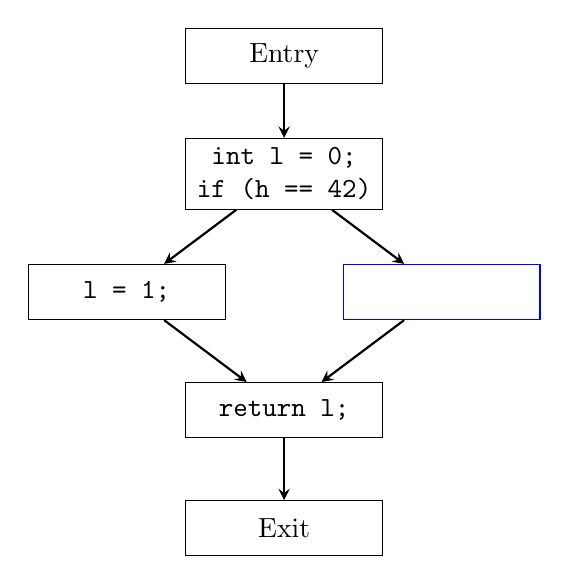
\begin{tikzpicture}
                \tikzstyle{node} = [rectangle, minimum width=2.5cm, minimum height=.7cm, text centered, draw=black, node distance=1.5cm]
                \tikzstyle{arrow} = [thick,->,>=stealth]
                
                \node (entry) [node] {Entry};
                \node (b1) [node, below of=entry, align=center] {\texttt{int l = 0;} \\ \texttt{if (h == 42)}};
                \node (b2) [node, below of=b1, xshift=-2cm] {\texttt{l = 1;}};
                \node (b22) [node, below of=b1, xshift=+2cm, draw = blue] {};
                \node (b3) [node, below of=b2, xshift=+2cm] {\texttt{return l;}};
                \node (exit) [node, below of=b3] {Exit};

                \draw [arrow] (entry) -- (b1);
                \draw [arrow] (b1) -- (b2);
                \draw [arrow] (b1) -- (b22);
                \draw [arrow] (b2) -- (b3);
                \draw [arrow] (b22) -- (b3);
                \draw [arrow] (b3) -- (exit);
            \end{tikzpicture}
        \caption{Control Flow Graph\\The highlighted node was inserted to split a critical edge.}
        \label{fig:cfg}
    \end{subfigure}\hfill
    \begin{subfigure}[t]{.45\textwidth}
        \centering
        \begin{tikzpicture}
            \tikzstyle{node} = [ellipse, minimum width=2.5cm, minimum height=.7cm, text centered, draw=black, node distance=2cm]
            \tikzstyle{arrow} = [thick,->,>=stealth]
            
            \node (b1) [node] {\texttt{int l = 0;}};
            \node (b2) [node, below left of=b1] {\texttt{h == 42}};
            \node (b3) [node, below of=b2] {\texttt{l = 1;}};
            \node (b4) [node, below right of=b3] {\texttt{return l;}};

            \draw [arrow] (b1) -- (b4);
            \draw [arrow, blue] (b2) -- (b3);
            \draw [arrow] (b3) -- (b4);
        \end{tikzpicture}
        \caption{Program Dependence Graph\\The black edges are data dependencies, while blue edges show control dependencies}
        \label{fig:pdg}
    \end{subfigure}
    \caption{Different graph representations for the program snippet in \ref{fig:ifEx}}
\end{figure}

\section{Program Slicing}

\section{Model Counting}

Given a propositional formula $F$, the model counting problem (\#SAT) is the problem of finding the number of distinct variable assignments for $F$, for which $F$ evaluates to true \cite{biere09}. So the solution for the formula shown in  \ref{fig:satEx} is \#F = 3, with the only non-fulfilling variable assignments being $\{ x = \mttt, y = \mfff\}, \{x = \mttt, y = \mttt\}$ and  $\{x = \mfff, y = \mfff\}$.

\#SAT is a generalization of the SAT problem and falls into the \#P-complete complexity class, as demonstrated by Valiant in \cite{valiant79}.

Early exact model counting techniques, such as \cite{birnbaum99}, or the well-known tool sharpSAT \cite{thurley06} use a DPLL-style exploration of the solution space. Another class of model counters instead employ complex transformations to turn the given CNF formula into a different representation, which makes model counting a far easier problem. Common are transformations into \emph{binary decision diagrams} (\td{citation!}) or \emph{deterministic, decomposable negation normal form} \cite{darwiche04}.

\paragraph*{Approximate Model Counting}
State-of-the-art exact model counters scale to a couple of hundred variables.  This limit can be pushed to around 1,000 variables if we allow approximate solutions \cite{biere09}.
The first approximate \#SAT algorithm for DNF formulas was introduced by Luby and Karp in \cite{karp89} used Monte-Carlo techniques. This approach was extended to work on CNF formulas by Chakraborty, Meel and Vardi in \cite{chakraborty13}. Both procedures fall under category of $(\epsilon, \delta)$-counters: for $0 < \epsilon, \delta \leq 1$, the approximated solution $\#F_{approx}$ to the true solution of the problem \#F, lies in the interval $[(1 + \epsilon)^{-1} \#F, \: (1 + \epsilon) \#F]$ with a probability of $1 - \delta$ \cite{karp89,chakraborty13}.

\begin{figure}
    \centering
    $F := x \lor \lnot y$
    \caption{Propositional formula with 2 variables}
    \label{fig:satEx}
\end{figure}



\paragraph*{Projected Model Counting}
Given a set of propositional variables $\mathcal{V}$ and a propositional formula $F$ over $\mathcal{V}$, projected model counting (\#$\exists$SAT) is the problem of finding the number of assignments to a set of priority variables $\mathcal{P} \subseteq \mathcal{V}$, such that the assignment can be extended to an assignment over $\mathcal{V}$ that fulfills $F$. Considering the example from \ref{fig:satEx} and a priority set $\mathcal{P} = \{x\}$, the number of projected models is 2, with both possible assignments of $x$ being extendable to a fulfilling assignment over all variables by setting $y = \mfff$.

The problem is introduced by Aziz et.al. in \cite{aziz15}, along with a discussion of approaches to solve \#$\exists$SAT. \td{finish}

% Model Counting
% Complexity
% Hashing-based approaches
% Application to CNF
% (\epsilon, \delta) approximation / "Probably Approximately Correct"

%%% relevant for this section
% The Complexity of Enumeration and Reliability Problems (Valiant '79) -- \cite{valiant79}
% A scalable approximate model counter (chakraborty '13) -- \cite{chakraborty13}
